\documentstyle[epsfig]{aipproc}

\widowpenalty=1000

\begin{document}

\title{Structure of the Goldstone Bosons}

\author{Roy J. Holt and Paul E. Reimer}
\address{Argonne National Laboratory\\
         Argonne, Illinois  60439}

\maketitle

\begin{abstract}
The feasibility of measuring the pion and kaon structure functions has
been investigated.  A high luminosity electron-proton collider would
make these measurements feasible.  Also, it appears feasible to
measure these structure functions in a nuclear medium.  Simulations
using the RAPGAP Monte Carlo of a possible pion structure function
measurement will be presented.
\end{abstract}

\section*{Introduction}


The light mesons, especially the pion, have a central role in nuclear
physics and nucleon structure.  The light meson spectrum is believed
to be the consequence of a dynamically broken chiral symmetry and are
regarded as the Goldstone bosons of quantum chromodynamics.  Moreover,
the valence structure of the meson involves only a $q\overline{q}$
system, {\it i.e.} a two-body interaction.  Recently, several
contemporary theoretical calculations were performed for the pion
structure function.  These calculations were based on a
Dyson-Schwinger Equation (DSE) model\cite{hecht}, a Nambu Jona-Lasinio
model (NJL)\cite{shigetani}, and chiral quark models\cite{weise}.  In
addition, the first few moments of the pion structure function were
determined from a lattice gauge calculations\cite{best}.  The kaon
structure function has been calculated within the framework of the NJL
model\cite{shigetani}.

According to the chiral quark model, there should be a large
difference between the sea quarks in the nucleon and those of the
pion.  In particular, the momentum fraction carried by the sea quarks
in the pion is expected\cite{weise} to be substantially larger than
that in the nucleon.

In addition to the free pion structure function calculations, there
exists a calculation of the pion structure function in the nuclear
medium\cite{suzuki}.  This calculation makes use of the NJL model and
compares the result to the effect expected from Brown-Rho
scaling\cite{brown}.

The kaon structure function is particularly interesting since the
``heavy'' strange valence quark is expected to carry a larger part of
the kaon momentum than the $u$ or $d$ quark.  The theoretical
calculations\cite{shigetani} indicate that the probability to find a
$\overline{u}_v$ quark in the $K^-$ diminishes as $x$ increases,
indicating the presence of this mass effect.  Unfortunately, the
Drell-Yan data\cite{badier} are sufficiently poor that this feature is
not determined unambiguously.

The purpose of this report is to assess the feasibility of measuring
the pion structure function with a proposed\cite{bland} electron light
ion collider (EPIC).  In addition, a possible experiment to measure
the kaon structure function is discussed.  Finally, the feasibility of
measuring the pion and kaon structure functions in the nuclear medium
is discussed.


\section*{Previous Experiments}

The pion structure function was measured previously in a Drell-Yan
experiment\cite{conway} (E615) at Fermilab.  The results of this
experiment are shown in Fig.~\ref{fig1}.  The data extend from a Bjorken
$x_\pi$ of 0.2 to 0.98.  The statistical errors on the data below an
$x_\pi$ of 0.4 are rather large, while the errors at high $x_\pi$ are
surprisingly small.  Hecht {\it et al.} \cite{hecht} have shown that
the high $x_\pi$ data can only be explained by a functional form which
has a constant probability to find a valence quark in configuration
space.

\begin{figure} % fig 1
\centerline{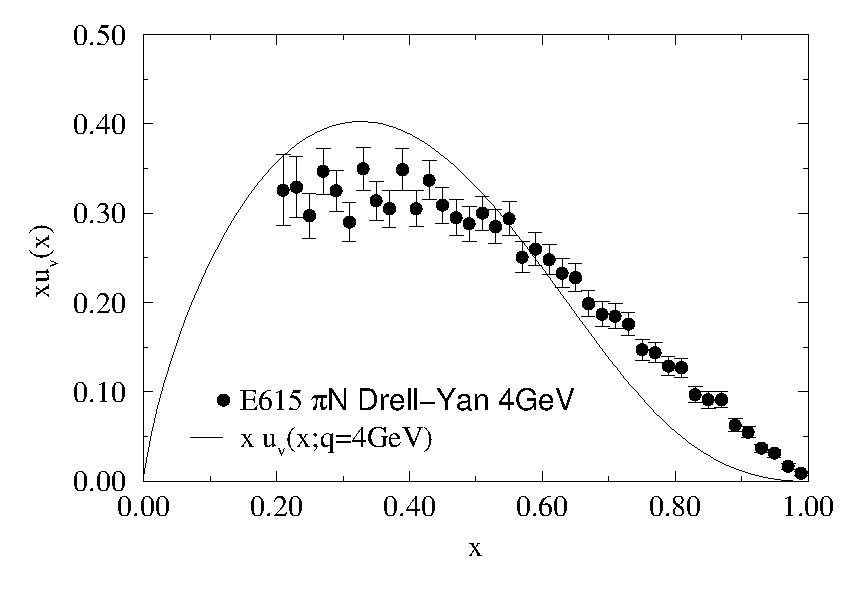
\epsfig{file=craig.eps,height=2.4in,width=3.5in}}
\caption{Existing data for the pion structure function from Drell-Yan
         scattering \protect\cite{conway}.  The solid curve represents
         a dynamical calculation~\protect\cite{hecht}. }
\label{fig1}
\end{figure}

In addition to the Drell-Yan data, there exist some recent quark
structure function data\cite{adloff} from HERA using deep inelastic
scattering from the pion cloud in the proton.  These data occur at
very low $x_\pi$.  Several theoretical analyses
\cite{pirner,holtmann,kopeliovich} have argued that the pi-nucleon
splitting function is known well enough to make reasonably accurate
measurements of the pion structure function.  The basic Feynman
diagram that occurs in these theoretical analyses is given in
Fig. \ref{fig2}.

\begin{figure} % fig 2
\centerline{\epsfig{file=feyn.eps}}
\vspace{10pt}

\caption{Deep inelastic scattering from the pion cloud surrounding a 
         proton.}

\label{fig2}
\end{figure}

Finally, dijet measurements\cite{dijet} were performed by the ZEUS
Collaboration at HERA.  In this experiment the dijets were detected in
the photoproduction regime and in coincidence with a forward-going
neutron.  The results are consistent with the simple one-pion exchange
model and may be a promising way to measure the valence part of the
pion structure function over a large $x_\pi$ range.

\section*{Simulation of a Collider Experiment}

The scattering process was simulated using the RAPGAP Monte Carlo
program~\cite{jung}.  RAPGAP models processes in which there is a
large rapidity gap between a fast outgoing nucleon and the remainder
of the inelastic scattering fragments.  These processes include DIS
from an exchanged pion or pomeron as illustrated in Fig.~\ref{fig2}.
A comparison of results from RAPGAP with HERA data show reasonable
agreement for fast outgoing neutrons \cite{adloff}.

\begin{figure}[b] % fig 3
\centerline{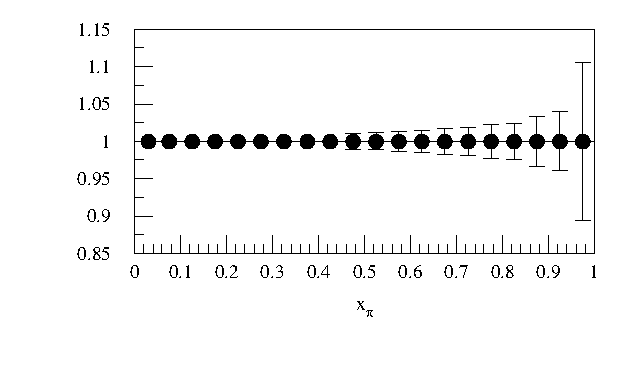
\epsfig{file=error.eps}}
\caption{Simulated errors for DIS events using a 5 GeV electron beam
         on a 25 GeV proton beam with a luminosity of
         $10^{32}\textrm{cm}^{-2}\textrm{s}^{-1}$ and $10^6\textrm{s}$
         of running.}
\label{errors}
\end{figure}

For a 5 GeV electron beam on a 25 GeV proton beam, RAPGAP calculates
22 nb cross section for the $eq\rightarrow e'q'$ process.  The
expected accuracy of the experiments was calculated using events in
which a ``spectator'' neutron was identified.  In general, the neutron
is scattered less than 50 mrad from the nominal proton beam axis.
Events were cut on $-q^2 > 1~\textrm{GeV}^2$.  An additional cut was
made to insure that the kinematics of the nucleon-pion system nearly
matched those of a na\"{\i}ve model in which a free pion is traveling
colinearly with a neutron.  This cut was made on the variable $x_L =
({\bf p}\cdot {\bf q}) / ({\bf p'}\cdot {\bf q})$, where ${\bf p}$,
${\bf p'}$ are the four momentum of the initial and final nucleons and
${\bf q}$ is the four momentum transfer of the virtual photon.  The
expected errors are shown in Fig. \ref{errors}.  A luminosity of
$10^{32}~\textrm{cm}^{-2}\textrm{s}^{-1}$ was assumed for a run
lasting $10^6~\textrm{s}$.  For the purposes of this report, detector
efficiency and acceptance were not simulated and a perfect detector
was assumed.


\section*{The Kaon Structure Function}

The $K^+$ structure function can be measured by considering deep
inelastic scattering from the kaon cloud surrounding a proton.  The
basic Feynman diagram would be the same as in Fig. 2 with the pion
replaced by a kaon and the neutron replaced by a $\Lambda$.  The
probability for scattering from the $K^+$ cloud surrounding the proton
should be comparable to that for the $\pi^+$ since the KN$\Lambda$
coupling constant is comparable to that of the $\pi$NN vertex.  In
fact, one would only expect about a factor of two reduction in the
vertex function for the kaon compared to the pion.

The difficulty with this process is in the detection of the $\Lambda$.
The $\Lambda$ decays predominantly (99\%) to a proton and a $\pi^-$.
Thus, a special forward proton spectrometer as well as a forward pion
spectrometer would be necessary.  This should be feasible since the
ZEUS and H1 experiments at HERA have already successfully employed
forward proton spectrometers.  When designing the ring magnets, one
should take into account the possibility of detecting both positively
and negatively charge forward going hadrons.  Simulations for this
part of the experiment would be necessary to optimize the detection
efficiency.

\section*{Pion Structure in the Nuclear Medium}

The question of pions in the nuclear medium continues to be an issue.
Neither Drell-Yan experiments\cite{drellyan} nor A(e,e'$\pi$) experiments
\cite{jackson} have
revealed the pion excess expected in nuclei.  It would be interesting
to determine whether the pion or kaon structure functions become
modified in a nuclear medium.  An electron light-ion collider should
render these studies feasible for nuclei up to $^4$He.  For the pion
case, the idea would be to detect all of the forward going nucleons
from the deep inelastic scattering from the pion.  In the case of a
deuterium target, for example, one would detect both forward going
neutrons or forward going protons, depending on whether the DIS
occurred from the $\pi^+$ or the $\pi^-$, respectively.

One of the main technical issues is whether the Fermi motion of the
nucleons obscures the measurement of the transverse momentum of the
nucleons.  The Fermi motion is comparable to the peak of the $p_T$
distribution from DIS on the pion cloud on a free proton.  Again,
simulations for this experiment would be necessary.

\section*{Summary}

In summary, a measurement of the pion structure function over a large
$x_\pi$ region was shown to be feasible with an electron proton
collider, where the electron energy is 5 GeV, the proton energy is 25
GeV, and the luminosity is 10$^{32}$ cm$^{-2}$s$^{-1}$.  A collider
may open up other very interesting possibilities such as a measurement
of the meson structure function in the nuclear medium or a measurement
of the kaon structure function.

\section*{Acknowledgments}

We wish to thank C. Roberts, G. Levman, M. Derrick and T.-S. H. Lee
for very useful discussions.  In addition, we thank H. Jung and
D. H. Potterveld for valuable assistance with RAPGAP.  This work was
supported by the U. S. Department of Energy, Nuclear Physics Division,
under contract No. W-31-109-ENG-38.

\begin{references}

\bibitem{hecht}Hecht, M. B., Roberts, C. D., Schmidt, S. M., preprint
        (2000), nucl-th/0008049.

\bibitem{shigetani}Shigetani, T., Suzuki, K., Toki, H. {\it Phys. Lett.}
         {\bf B308}, 383 (1993); Davidson, R. M., Arriola, E. Ruiz 
         {\it Phys. Lett} {\bf B348}, 163 (1995).

\bibitem{weise}Suzuki, K., Weise, W. {\it Nucl. Phys. } {\bf A634}, 
         141 (1998).

\bibitem{best}Best, C. {\it et al.} {\it Phys. Rev. } {\bf D56}, 2743 
         (1997).

\bibitem{suzuki}Suzuki, K. {\it Phys. Lett. } {\bf B368}, 1 (1996).

\bibitem{brown}Brown, G. E., Rho, M. {\it Phys. Rev. Lett. } {\bf 99},
         2720 (1991).

\bibitem{badier}Badier, J., {\it et al.} {\it Phys. Lett. } {\bf B93},
         354 (1980).

\bibitem{bland}Bland, L. C., Londergan, J. T., Szczepaniak, A. P.,
         editors, {\it Physics with a High Luminosity Polarized Electron
         Ion Collider}, Singapore: World Scientific, 1999, and
         references therein.

\bibitem{conway}Conway, J. S. {\it et al.} {\it Phys. Rev. } {\bf D39},
         39 (1989).

\bibitem{adloff}Adloff, C. {\it et al.} (H1 Collaboration) {\it Eur. 
         Phys. J. C } {\bf 6}, 587 (1999).

\bibitem{pirner}D'Alesio, U. and Pirner, H. J. {\it Eur. Phys. J. A }
         {\bf 7}, 109 (2000).

\bibitem{holtmann} Holtmann, H. {\it et al.} {\it Nucl. Phys.} 
         {\bf A569}, 631 (1996).

\bibitem{kopeliovich} Kopeliovich, H. {\it et al.} {\it Z. Phys.  } 
         {\bf C73}, 125 (1996).

%\bibitem{zeus} Zeus Collaboration, XXXth Int. Conf. on High Energy 
%         Physics, Osaka, preprint (2000).
 
\bibitem{dijet} Zeus Collaboration, XXXth Int. Conf. on High Energy 
         Physics, Osaka, preprint (2000).

\bibitem{jung} Jung, H., {\it Comp. Phys. Commun.} {\bf 86}, 147 (1995).

\bibitem{drellyan} Alde, D. M. {\it et al.} {\it Phys. Rev. Lett.} {\bf 64}, 
     2479 (1990).

\bibitem{jackson} Jackson, H. E. (NucPi Collaboration) {\it Sixteenth Int'l Conf.
on Few Body Systems } Taipei, preprint (2000).

\end{references}
 
\end{document}


